\input{../../common/slide-common-header.tex}

\newcommand{\orgNum}{0}
\newcommand{\orgTopic}{org meeting}
\newcommand{\orgKey}{syllabus, contacts}

\newcommand{\introNum}{1}
\newcommand{\introTopic}{introduction to multithreading}
\newcommand{\introKey}{concurrency, parallelism, agents, threads, scheduler, threading models, interleaving execution,  Amdahl's law, race condition, data race, deadlock, wait-for graph}

\newcommand{\basicNum}{2}
\newcommand{\basicTopic}{mutual exclusion}
\newcommand{\basicKey}{thread safety, concurrent consistency, mutual exclusion, critical section, deadlock-freedom, starvation, fairness, check-then-act, reentrancy, admission policy, code locking, data locking, lock splitting, lock ordering, dining philosophers problem}

\newcommand{\basicTwoNum}{3}
\newcommand{\basicTwoTopic}{signalling}
\newcommand{\basicTwoKey}{thread factory, executor, future, thread pooling, backoff policy, signalling, condition variable, lost signal, spurious wakeup, wait set admission policy, blocking queue, predicate invalidation, thread-starvation deadlock, resource deadlock}

\newcommand{\syncPrimitivesNum}{4}
\newcommand{\syncPrimitivesTopic}{advanced synchronization primitives}
\newcommand{\syncPrimitivesKey}{monitor, synchronized, completion service, thundering herd problem, wait morphing, countdown latch, semaphore, read-write lock, thread local, replication, snapshotting}

\newcommand{\patternsNum}{5}
\newcommand{\patternsTopic}{cancellation and interruption}
\newcommand{\patternsKey}{concurrent state machine, forced cancellation, cooperative cancellation, cancellation token, interruption, timeouts}

\newcommand{\reliabilityNum}{6}
\newcommand{\reliabilityTopic}{reliability}
\newcommand{\reliabilityKey}{documenting protocols and classes, concurrent invariants, assertions, stress testing, estimating bug probability, static and dynamic checks, scheduling randomization and determinisation, model checking}

\newcommand{\foundationsNum}{7}
\newcommand{\foundationsTopic}{theoretical foundations of concurrency}
\newcommand{\foundationsKey}{timeline, events, precedence, 2-thread mutual exclusion, deadlock freedom, starvation freedom, N-thread mutual exclusion, sequential objects and specifications, concurrent objects, linearizability}

\newcommand{\foundationsPlusNum}{8}
\newcommand{\foundationsPlusTopic}{progress guarantees, concurrent operations hierarchy, consensus number}
\newcommand{\foundationsPlusKey}{obstruction-free, lock-free, wait-free, safe register, regular register, atomic register, register snapshot, consensus number}

\newcommand{\atomicsNum}{9}
\newcommand{\atomicsTopic}{introduction to atomics}
\newcommand{\atomicsKey}{read-modify-write, get-and-add, compare-and-swap, spin lock, lock-free stack, ABA problem}

% TODO: taxonomy of queues, 

\newcommand{\cacheCoherencyNum}{10}
\newcommand{\cacheCoherencyTopic}{cache coherency}
\newcommand{\cacheCoherencyKey}{cache memory hierarchy, cache coherency protocol, store-buffer, load-buffer, invalidate-queue, memory barrier, hardware memory model, weak memory model, litmus tests}

\newcommand{\langMMNum}{11}
\newcommand{\langMMTopic}{language memory model}
\newcommand{\langMMKey}{compiler optimizations, compiler barriers, language memory model, strict consistency, threads cannot be implemented as a library, visibility, volatile}

\newcommand{\advancedConcurrencyNum}{12}
\newcommand{\advancedConcurrencyTopic}{advanced locking}
\newcommand{\advancedConcurrencyKey}{Anderson Queue Lock, CLH, MCS, check-then-act, spin-then-park}

% TODO: work distribution, work stealing, taxonomy of parallel problems, single LIFO cell optimization, RAT

\newcommand{\userSpaceThreadingNum}{13}
\newcommand{\userSpaceThreadingTopic}{user-space threading}
\newcommand{\userSpaceThreadingKey}{berkley socket, blocking and non-blocking IO, callback-hell, async-await, continuation-passing-style, fibers/coroutines/green threads, stackful vs stackless}

\newcommand{\concurrentQueuesNum}{14}
\newcommand{\concurrentQueuesNumTopic}{concurrent queues}
\newcommand{\concurrentQueuesNumKey}{queue as mutex, strong FIFO, per-producer FIFO, bounded/unbounded queue, SPSC, MPSC, SPMC, MPMC, total/partial/synchronous API, lock-free queue, ring buffer for bounded queues, concurrent dequeue, work stealing}

% \newcommand{\designNum}{13}
% \newcommand{\designTopic}{designing concurrent systems}
% \newcommand{\designKey}{park/unpark, synchronizer, futex/wait-on-address, plan9 approach, race-finders, ForkJoinPool/CoroutineCarriers/UIthread, observability, structured concurrency}

% \newcommand{\frameworksAndDistributedNum}{14}
% \newcommand{\frameworksAndDistributedTopic}{multi-agent systems}
% \newcommand{\frameworksAndDistributedKey}{auto-parallelization languages and frameworks, semi-automatic synchronization, distributed systems, consensus protocols}


\newcommand{\thisLectureNum}{\reliabilityNum}

\title[]{Lecture \thisLectureNum: \reliabilityTopic}
\subtitle[]{\reliabilityKey}
\author[]{Alexander Filatov\\ filatovaur@gmail.com}

\date{}

\newcommand{\alarmOne}{\textbf{Alarm bell №1}: we do not know how to formalize \textit{consistency}}
\newcommand{\alarmTwo}{\textbf{Alarm bell №2}: non-determinism caused by CPU speed and scheduler decisions}
\newcommand{\alarmThree}{\textbf{Alarm bell №3}: concurrent problems could be OS/CPU/compiler/environment-specific}
\newcommand{\alarmFour}{\textbf{Alarm bell №4}: decreasing concurrent bug probability requires excessive computing power}
\newcommand{\alarmFive}{\textbf{Alarm bell №5}: we do not know how to guarantee ''zero concurrent bug'' property}
\newcommand{\alarmSix}{\textbf{Alarm bell №6}: static analysis lack run-time knowledge (false positives)}
\newcommand{\alarmSeven}{\textbf{Alarm bell №7}: dynamic analysis works for particular execution trace only}

\begin{document}

\begin{frame}
  \titlepage
  \url{https://github.com/Svazars/parallel-programming/blob/main/slides/pdf/l\thisLectureNum.pdf}
\end{frame}

\begin{frame}{In previous episodes}

Concurrent coordination concepts:
\begin{itemize}
    \item Mutual exclusion, Signalling, Group-level concurrency, Separation of threads and tasks
    \item Cancellation, interruption
\end{itemize}

Concurrent data structures:
\begin{itemize}
    \item \texttt{Lock}, \texttt{Condition}, \texttt{Monitor}, \texttt{CountDownLatch}, \texttt{Semaphore}, \texttt{ReadWriteLock}
\end{itemize}

Concurrent programming patterns:
\begin{itemize}
    \item Code locking, Data locking, Lock splitting, Exponential backoff
    \item Replication, Snapshotting, Concurrent state machine 
\end{itemize}

Concurrent software problems:
\begin{itemize}
    \item Race condition, data race, deadlock
    \item Lost signal, predicate invalidation, spurious wakeup, fairness    
    \item Thundering herd, oversubscription
\end{itemize}

\end{frame}

\newcommand{\painpointsslide}{
\begin{frame}{Pain points}

\begin{itemize}
  \item Unpredicatable speed of execution
  \item Arbitrary "whole program control flow"
  \begin{itemize}
    \item \texttt{Thread.start} looks like \texttt{goto}
  \end{itemize}
  \item Arbitrary "thread-specific control flow"
  \begin{itemize}
    \item timeout, notification, interruption, spurious wakeup
  \end{itemize}

  \item Limited composability of modules 
  \begin{itemize}
    \item locking policy is not clear
    \item lock ordering hidden by virtual methods
    \item exposed \texttt{synchronized}
    \item non-documented thread-safety    
  \end{itemize}

  \item Hard to diagnose performance problems 
  \begin{itemize}
    \item underutilization, priority inversion, thundering herd, scalability 
  \end{itemize}

  \item It is \textbf{too easy} to introduce a race condition
  \begin{itemize}
    \item it is \textbf{too hard} to find it on review, during testing, debug on production system
  \end{itemize}
\end{itemize}
\end{frame}  
}

\painpointsslide

\questiontime{Concurrency is a very complicated programming domain. What could we do to simplify our programming life?}


\begin{frame}{Lecture plan}
\tableofcontents
\end{frame}

\section{Concurrent invariants}
\showTOC

\questiontime{How user of your program will know its features and limitations?}

\begin{frame}[t]{Documentation}

Reading \only<3->{and \textbf{writing}} the docs:
\begin{itemize}
  \item Thread-safety of a class
  \item How to use class to avoid inconsistent state (e.g. \texttt{try-finally} for \texttt{Lock})
  \item Blocking operations
  \item Locking policy
  \item Admission policy
  \item Inheritance policy
\end{itemize}

\pause

\only<2> {Writing the docs:}

\pause
\pause

\texttt{java.util.concurrent} is a good source for inspiration

\end{frame}

\questiontime{Nobody reads the documentation! How could I \textbf{enforce} usage patterns of my class?}


\begin{frame}[fragile,t]{Invariants checking}

Single-threaded code crashes with \texttt{ConcurrentModificationException}\footnote{\tiny\url{https://stackoverflow.com/questions/3184883/concurrentmodificationexception-for-arraylist}}:

\begin{minted}{java}
void foo(List<X> list) {  
  for (X x : list) {
    if (!x.isValid()) list.remove(x);
  }
}
\end{minted}

\pause

It is intended behaviour\footnote<2->{\tiny\url{https://docs.oracle.com/en/java/javase/11/docs/api/java.base/java/util/ArrayList.html}}
\begin{quote}
  The iterators returned by this class's `iterator` ... are fail-fast: if the list is structurally modified at any time after the iterator is created, in any way except through the iterator's own `remove` or `add` methods, the iterator will throw a `ConcurrentModificationException`. Thus, in the face of concurrent modification, the iterator fails quickly and cleanly, rather than risking arbitrary, non-deterministic behavior at an undetermined time in the future. 
\end{quote}

\end{frame}

\questiontime{How to implement such consistency check (collection is not modified while iterated)?}

\begin{frame}[fragile,t]{Invariants checking}

Advantages:
\begin{itemize}
  \item Contract is enforced by implementation rather by javadoc
  \item Fail-fast behaviour speed-ups debugging
  \item Type of exception and stacktrace information help to debug large systems 
\end{itemize}

Disadvantages:
\begin{itemize}
  \item Performance overheads
  \item Incompleteness (impossible to cover all misuses)
  \item Affects even single-threaded programs
\end{itemize}
\end{frame}

\questiontime{How could we implement lightweight or zero-cost checks?}

\begin{frame}[fragile,t]{Assertions}

Assertions\footnote{\tiny\url{https://docs.oracle.com/javase/specs/jls/se11/html/jls-14.html#jls-14.10}}:

\begin{minted}{java}
void foo(ArrayList<String> list) {
  assert list != null;
  assert list.size() > 0;
}
\end{minted}

\pause

\begin{quote}
Typically, assertion checking is enabled during program development and testing, and disabled for deployment, to improve performance.
\end{quote}

\pause

\begin{quote}
Because assertions may be disabled, programs must not assume that the expressions contained in assertions will be evaluated. Thus, these boolean expressions should generally be free of side effects. 
\end{quote}

\pause

\begin{quote}
In light of this, assertions should not be used for argument checking in public methods. Argument checking is typically part of the contract of a method, and this contract must be upheld whether assertions are enabled or disabled.
\end{quote}

\end{frame}


\begin{frame}[fragile,t]{Assertions}

\begin{itemize}
  \item Could be enabled/disabled without recompilation of Java program\footnote{\tiny\url{https://docs.oracle.com/javase/8/docs/technotes/guides/language/assert.html}}
  \begin{itemize}
    \item Many guidelines enforce \texttt{java -ea -esa -jar production.jar ...}
  \end{itemize}

  \item Should be used for checking \textbf{internal consistency} (violation of programmer's intent), not \textbf{external consistency} (e.g validation of user input)

  \item Perfect choice to make concurrent programs fail-fast
  \begin{itemize}
    \item Use \texttt{-enablesystemassertions} to fail-fast on subtle data races inside improperly used classes from standard library (e.g. unsynchronized access to \texttt{ArrayList})
  \end{itemize}
\end{itemize}
\end{frame}


\begin{frame}[fragile,t]{Optional heavyweight checks}

\begin{minted}{java}
class MyLinkedList {
  private int cachedLength;
  private Node head;
  private int length() {
    int size = 0;
    for (Node n = this.head; n != null; n = n.next, size++) {}
    return size;
  }
  public void add(Node e) {
    e.next = this.head;
    this.head = e;
    cachedLength++;
    assert cachedLength == length();
  }
}
\end{minted}

\end{frame}

\begin{frame}[fragile,noframenumbering,t]{Optional heavyweight checks}

\begin{minted}{java}
class MyLinkedList {
  private int cachedLength;
  private Node head;
  private int length() {
    int size = 0;
    for (Node n = this.head; n != null; n = n.next, size++) {}
    return size;
  }
  public void add(Node e) {
    e.next = this.head;
    this.head = e;
    cachedLength++;
    assert heavyChecksDisabled() || cachedLength == length();
  }
}
\end{minted}
\end{frame}


\begin{frame}[t]{Optional heavyweight checks}

\begin{itemize}
  \item Could find non-local data inconsistency
  \item May be prohibitively slow for production workloads
  \item Distort concurrent execution patterns (change probability of race condition)
  \item May be designed to provide detailed information about failure
\end{itemize}
\end{frame}


\begin{frame}[t]{Summary: invariants}

\begin{itemize}
  \item Invariants help to make better contracts and design more reliable programs
  \item Report failed external contracts with detailed exceptions
  \item Check internal contracts with lightweight checks (e.g. optional \texttt{assert}s)
  \item Consider using heavyweight checks for special modes of execution (e.g. debug builds)
\end{itemize}

\pause

You can not start checking for correctness until you understand 
\begin{itemize}
  \item allowed
  \item forbidden
\end{itemize}
result of your algorithm or data structure.
\end{frame}

\questiontime{What are the main requirements for thread-safe code?}

\begin{frame}{Concurrent invariants and thread safety}

Some validity rules are obvious and trivial:
\begin{itemize}
  \item Does not fail with \texttt{AssertionError}, \texttt{NullPointerExcepiton} ...
  \item Deadlock never happens, data race never happens ...
  \item ...
\end{itemize}

\pause

Describing behaviour in multithreaded environment requires additional effort:
\begin{itemize}
  \item After data is \texttt{add}ed to thread-safe collection, some other thread eventually could \texttt{remove} it
  \pause
  \item only once
\end{itemize}

\pause

Concurrent consistency could be hard to explain and check\footnote<4->{\tiny\url{https://en.wikipedia.org/wiki/Sequential_consistency}}:
\begin{quote}
  ... the result of any execution is the same as if the operations of all the processors were executed in some sequential order, and the operations of each individual processor appear in this sequence in the order specified by its program.
\end{quote}

\pause

\alarmOne

\end{frame}

\questiontime{How do you \textbf{automatically} check that your program does not fail with assertions?}

\section{Testing}
\showTOC

\subsection{Unit testing}

\begin{frame}{Unit testing}

Focus on safety (correctness).

\pause

\begin{itemize}
  \item All single-threaded scenarios
  \item Basic multi-threaded scenarios
  \item Advanced multi-threaded scenarios with custom scheduling (insertion of \texttt{Thread.sleep})
\end{itemize}

\pause
Goals:
\begin{itemize}
  \item coverage
  \item regression tests
  \item supplementary documentation for intended and forbidden usages
\end{itemize}

\pause
Tools:
\begin{itemize}
  \item JUnit\footnote<4->{\tiny\url{https://junit.org}} 
\end{itemize}

\end{frame}

\questiontime{Unit tests are small and fast. How to ensure concurrent software properly works under pressure?}

\subsection{Stress testing}
\showTOCSub

\begin{frame}[t,fragile]{JCStress}

{\small\url{https://github.com/openjdk/jcstress}}

\begin{minted}{java}
@JCStressTest
@Outcome(id = "1, 2", expect = ACCEPTABLE, desc = "actor1 -> actor2.")
@Outcome(id = "2, 1", expect = ACCEPTABLE, desc = "actor2 -> actor1.")
@State
public class TestConcurrentIncrements {
    int v;
    @Actor public void actor1(II_Result r) { r.r1 = ++v; }
    @Actor public void actor2(II_Result r) { r.r2 = ++v; }
}
\end{minted}
\end{frame}

\begin{frame}[t,fragile,noframenumbering]{JCStress}
\begin{minted}{java}
@JCStressTest
@Outcome(id = "1, 2", expect = ACCEPTABLE, desc = "actor1 -> actor2.")
@Outcome(id = "2, 1", expect = ACCEPTABLE, desc = "actor2 -> actor1.")
@State
public class TestConcurrentIncrements {
    int v;
    @Actor public void actor1(II_Result r) { r.r1 = ++v; }
    @Actor public void actor2(II_Result r) { r.r2 = ++v; }
}
\end{minted}

\begin{minted}{text}
  RESULT     SAMPLES     FREQ      EXPECT  DESCRIPTION
    1, 1     120,616    0.52%   Forbidden  No default case provided
    1, 2  22,993,014   99.01%  Acceptable  actor1 -> actor2.
    2, 1     108,661    0.47%  Acceptable  actor2 -> actor1.
\end{minted}
\end{frame}

\begin{frame}[t,fragile,noframenumbering]{JCStress}

\begin{minted}{java}
@JCStressTest
@Outcome(id = "1, 1", expect = ACCEPTABLE_INTERESTING, desc = "Data race")
@Outcome(id = "1, 2", expect = ACCEPTABLE, desc = "actor1 -> actor2.")
@Outcome(id = "2, 1", expect = ACCEPTABLE, desc = "actor2 -> actor1.")
@State
public class TestConcurrentIncrements {
    int v;
    @Actor public void actor1(II_Result r) { 
      int tmp = v; tmp = tmp + 1; v = tmp; r.r1 = tmp;
    }
    @Actor public void actor2(II_Result r) { 
      int tmp = v; tmp = tmp + 1; v = tmp; r.r2 = tmp;
    }
}
\end{minted}
\end{frame}

\begin{frame}[t,fragile]{Homework: recording rare events}

{\small\url{https://github.com/Svazars/parallel-programming/tree/main/hw/block1/6.1}}
\begin{homeworkmail}{Task 6.1}
    \begin{itemize}
        \item Get familiar with JCStress
        \item Run stress test with 5 actors and single arbiter, explain results
    \end{itemize}
\end{homeworkmail}
\end{frame}


\begin{frame}[t,fragile]{Stress testing}
Advantages:
\begin{itemize}
  \item Finds bugs in concurrent programs
\end{itemize}

\pause
Disadvantages:
\begin{itemize}
  \item Finds bugs in concurrent programs \textbf{probabilistically}
\end{itemize}
\end{frame}


\begin{frame}[t,fragile]{Finding visibility bugs}
\begin{minted}{java}
@Outcome(id = "0, 0", expect = ACCEPTABLE, desc = "actor2  ->actor1")
@Outcome(id = "1, 0", expect = ACCEPTABLE, desc = "actor1.x->actor2->actor1.y")
@Outcome(id = "1, 1", expect = ACCEPTABLE, desc = "actor1  ->actor2")
@Outcome(id = "0, 1", expect = ACCEPTABLE_INTERESTING, desc = "???")
public class StrangeOrdering {
    int x; int y;
    @Actor public void actor1() { 
      x = 1;
      y = 1;
    }
    @Actor public void actor2(II_Result r) { 
      r.r2 = y;
      r.r1 = x;
    }
}
\end{minted}
\end{frame}

\questiontime{Why we could observe result that does not conform to any interleaving?}

\begin{frame}[t,fragile]{Stress testing}
Advantages:
\begin{itemize}
  \item Finds bugs in concurrent programs
  \item Finds bugs in concurrent programs caused by compiler optimizations
  \pause
  \begin{itemize}
    \item VM internals, OS scheduling, environment specifics ...
  \end{itemize}
\end{itemize}

\pause
Disadvantages:
\begin{itemize}
  \item Finds bugs in concurrent programs \textbf{probabilistically}
  \pause 
  \item Finds bugs in concurrent programs run in \textbf{particular} environment
\end{itemize}
\end{frame}


\begin{frame}[t,fragile]{Homework: recording ''impossible'' events}

{\small\url{https://github.com/Svazars/parallel-programming/tree/main/hw/block1/6.2}}
\begin{homeworkmail}{Task 6.2}
    \begin{itemize}
        \item Create stress-test equivalent to Task 1.3
        \item Find out possible concurrent results experimentally
        \item Check if all of them could be explained by interleaving model
    \end{itemize}
\end{homeworkmail}
\end{frame}

\begin{frame}[t,fragile]{Concurrent reliability is hard}

\begin{itemize}
  \item \alarmOne
  \item \alarmTwo
  \item \alarmThree
\end{itemize}
\end{frame}

\questiontime{Concurrency is hard! How many tests do I need to ensure my program is reliable?}

%\begin{frame}[t]{Performance testing}
%
%Focus on performance (resource utilization).
%
%\pause
%
%\begin{itemize}
%  \item Undersubscription because of critical sections
%  \item Oversubscription because of misconfigured thread pools
%  \item Inefficient contended execution path
%  \item Progress problems (livelock, priority inversion, starvation)
%\end{itemize}
%
%\pause
%
%Key metrics:
%\begin{itemize}
%  \item Throughput
%  \item Latency distribution
%  \item Resource leaks (objects, thread-local memory, thread handles, caches ...)
%  \item Scalability
%\end{itemize}
%
%\end{frame}
%
%
%\begin{frame}[t,noframenumbering]{Stress testing}
%Focus on performance (resource utilization).
%
%Key metrics:
%\begin{itemize}
%  \item Throughput, Latency, Resource utilization, Scalability
%\end{itemize}
%
%\pause
%Tools:
%\begin{itemize}
%  \item Java Microbenchmark Harness (JMH)\footnote<2->{\tiny\url{https://github.com/openjdk/jmh}}
%  \item Lincheck\footnote<2->{\tiny\url{https://github.com/JetBrains/lincheck}}
%\end{itemize}
%
%\pause
%Caveats: 
%\begin{itemize}
%  \item high-quality performance analysis requires years of low-level expertise
  %\item "We should forget about small efficiencies, say about 97\% of the time: premature optimization is the root of all evil. Yet we should not pass up our opportunities in that critical 3\%"
%\end{itemize}
%\end{frame}


%\subsection{Execution trace analysis}
%\showTOCSub
%
%\begin{frame}[fragile]{Execution trace analysis: idea}
%
%\begin{verbatim}
%  Timestamp: 1000400, Thread A: X.lock   (success)
%  Timestamp: 1000405, Thread B: Y.lock   (success)
%  Timestamp: 1000408, Thread A: X.lock   (success)
%  Timestamp: 1000411, Thread B: X.lock   (block)
%  Timestamp: 1000415, Thread A: Y.lock   (block)
%\end{verbatim}
%
%\pause
%
%\textt{Thread A} owns \texttt{X}, awaits for \texttt{Y}
%
%\textt{Thread B} owns \texttt{Y}, awaits for \texttt{X}
%
%\end{frame}
%
%
%\begin{frame}[fragile]{Examples of nontrivial consistency}
%
%\begin{verbatim}
%  Timestamp: 1, Thread A: list.add(User(1))
%  Timestamp: 2, Thread B: list.add(User(2))
%  Timestamp: 3, Thread C: list.removeAny(), result = User(2)
%  Timestamp: 3, Thread D: list.removeAny(), result = null
%  Timestamp: 5, Thread A: list.removeAny(), result = User(2)
%\end{verbatim}
%
%\pause
%
%Where is \texttt{User(1)}?
%
%\pause
%
%Why \texttt{User(2)} was removed twice?
%
%\end{frame}
%
%\begin{frame}{Execution trace analysis}
 %
% \begin{itemize}
%   \item Use \textbf{monotonic} stamps\footnote{\tiny\texttt{CLOCK\_MONOTONIC} \url{https://linux.die.net/man/3/clock_gettime}}
%   \pause
%   \begin{itemize}
     %\item \texttt{System.currentTimeMillis()} is \textbf{not} monotonic, be ready to time travel\footnote<2->{\tiny\url{https://shipilev.net/blog/2014/nanotrusting-nanotime/}}
%
%     \pause
%     \item \texttt{static synchronized long stamp() \{ return ++counter; \}} is safe approximation
%   \end{itemize}
 %
%   \pause
 %
%   \item Define obvious consistency violations
%   \begin{itemize}
%     \item Thread-safe collection cannot return \texttt{null} in moment \texttt{t2} if element was added at \texttt{t1 < t2}
%     \item Thread-safe collection cannot remove the same element twice if it was added only once
%     \item ...
%   \end{itemize}
 %
%   \pause
%   \item Collect execution trace (e.g. log file) from some scenario and check validity
 %
%   \pause
   %\item You could implement simple "reference solution"\ and check that it provides the same result on given execution trace\footnote<6->{\tiny\url{https://www.amazon.science/publications/using-lightweight-formal-methods-to-validate-a-key-value-storage-node-in-amazon-s3}}
% \end{itemize}
 %
%\end{frame}

% TODO: \textbf{Alarm bell №3}: we do not know how to control scheduling decisions to explore potential erroneous traces.

% \questiontime{How could I check that requirements for my data structure are complete, consistent, strong enough/weak enough?}
% \questiontime{How could I check that requirements for my data structure are complete, consistent, strong enough/weak enough? 
% Reconsider your answer after Lecture~\foundationsPlusNum.
% }

%\subsection{Test design to increase bug probability}
%\showTOCSub
%
%\begin{frame}{Common errors}
%
%\pause
%\begin{itemize}
%  \item Use delays (e.g. \texttt{Thread.sleep(100)}) to ensure that "other thread done something"
%  \begin{itemize}
%    \item use synchronized state variables, \texttt{CountDownLatch} or monitors
%  \end{itemize}
%
%  \pause
%  \item Use too strict assertions that trigger false-positive test failures
%  \begin{itemize}
%    \item formalize invariants, drop irrelevant constraints
%  \end{itemize}
%
%  \pause
%  \item Test scenarios are missing execution patterns so could not detect some race conditions
%  \begin{itemize}
%    \item use tests with custom scheduling and aim to 100\% coverage
%  \end{itemize}
%
%  \pause
%  \item Test scenarios are missing some essential consistency checks (e.g. because of mocking)
%  \begin{itemize}
%    \item enable some lightweight fail-fast checks on production system
%    \item validate execution trace from production system
%  \end{itemize}
%
%  \pause
%  \item Ignorance of tools
%  \begin{itemize}
%    \item use test generators (property testing, fuzzers, lincheck)
%    \item use properly designed concurrency stress systems (JMH, jcstress)
%    \item do not use tools that you do not understand \pause(ChatGPT may block your skill growth)
%  \end{itemize}
%
%  \pause
%  \item Obsessive perfectionism
%  \begin{itemize}
%    \item formalize QA criteria and limit investments into testing
%  \end{itemize}
%
%\end{itemize}
%\end{frame}


%\begin{frame}[fragile]{Common errors: sample v1}
%
%\begin{minted}{java}
%static int x = 0; static Object lock = new Object();
%void thread_1() {
%  synchronized(lock) {
%    assert x == 0;
%    lock.wait();
%    assert x == 1;
%  }
%}
%void thread_2() {
%  sleep(100); // allow thread_1 to grab lock
%  synchronized(lock) {
%    x++;
%    lock.notify();
%  }
%}
%\end{minted}
%\end{frame}
%
%\begin{frame}[fragile,noframenumbering]{Common errors: sample v2}
%
%\begin{minted}{java}
%static int x = 0; static Object lock = new Object();
%void thread_1() {
%  synchronized(lock) {
%    assert x == 0;
%    lock.wait();
%    assert x == 1;
%  }
%}
%void thread_2() {
%  // sleep(100);
%  synchronized(lock) {
%    x++;
%    lock.notify();
%  }
%}
%\end{minted}
%\end{frame}
%
%\begin{frame}[fragile,noframenumbering]{Common errors: sample v3}
%
%\begin{minted}{java}
%static int x = 0; static Object lock = new Object();
%void thread_1() {
%  synchronized(lock) {
%    // assert x == 0;
%    lock.wait();
%    assert x == 1;
%  }
%}
%void thread_2() {
%  // sleep(100);
%  synchronized(lock) {
%    x++;
%    lock.notify();
%  }
%}
%\end{minted}
%\end{frame}
%
%\begin{frame}[fragile,noframenumbering]{Common errors: sample v4}
%
%\begin{minted}{java}
%static int x = 0; static Object lock = new Object();
%void thread_1() {
%  synchronized(lock) {
%    // assert x == 0;
%    if (x == 0) lock.wait();
%    assert x == 1;
%  }
%}
%void thread_2() {
%  // sleep(100);
%  synchronized(lock) {
%    x++;
%    lock.notify();
%  }
%}
%\end{minted}
%\end{frame}

\subsection{Bug probability estimation}
\showTOCSub

\begin{frame}[t]{Validation: required mindset}

"Is parallel programming hard, and, if so, what can you do about it?" (a.k.a. perfbook)\footnote{\tiny\url{https://github.com/paulmckrcu/perfbook}}

Chapter 11 "Validation":

\pause

\begin{itemize}
         \item The only bug-free programs are trivial programs
  \pause \item A reliable program has no known bugs
\end{itemize}

\pause
Conclusion: 
\begin{itemize}
    \pause \item any reliable non-trivial program contains at least one bug that you do not know about
\end{itemize}
\end{frame}

\questiontime{If a tree falls in a forest and no one is around to hear it, does it make a sound?}

\questiontime{If a program has erroneous execution trace which never happens in practice, does it count as a bug?}

\begin{frame}{Enough is enough: estimate bug probability}

We will discuss the simplest discrete test scenario:
\begin{itemize}
  \item Individual test run either fails or successfully finishes\footnote{Continuous test example: run 1 minute under heavy contention, ensure no exception happen}
\end{itemize}

\pause
Probability of single failure $f$ (e.g. $0.1$, 10\%)

\pause
Probability of single success  $1 - f$ (e.g. $0.9$, 90\%)

\pause
Probability n repeats will succeed $S_n=(1-f)^n$

\pause
Probability of failure $F_n=1-(1-f)^n$

\pause
"How many times should we run the test to cause the probability of failure to rise above 99\%?" \pause

$$n=\frac{log(1-F_n)}{log(1-f)}$$

% f=0.1  and conf 99% -> 44 runs
% f=0.01 and conf 99% -> 458 runs

\end{frame}


\begin{frame}{Be careful. It is real world out there.}

\begin{itemize}
  \item As of 2017 Linux kernel was estimated to have more than 20 billion instances running
  \item Bug that occurs once every million years on a single system will be encountered more than 
  \begin{itemize}
    \pause \item 50 times per day
  \end{itemize}
\end{itemize}

\pause

Any mission-critical software for
\begin{itemize}
  \item health\footnote<3->{\tiny\url{https://en.wikipedia.org/wiki/Therac-25}}
  \item aerospace\footnote<3->{\tiny\url{https://en.wikipedia.org/wiki/Ariane_flight_V88}}
  \item military\footnote<3->{\tiny\url{https://devblogs.microsoft.com/oldnewthing/20180228-00/?p=98125}}
\end{itemize}
is also not satisfied with "just testing".
\end{frame}

\begin{frame}[t,fragile]{Concurrent reliability is hard}
\begin{itemize}
  \item \alarmOne
  \item \alarmTwo
  \item \alarmThree
  \item \alarmFour
  \item \alarmFive
\end{itemize}
\end{frame}

\questiontime{There are a lot of programs that operate on other programs: compilers, linters, debuggers ... Any help with prevention of concurrent bugs?}

\section{Tooling}
\showTOC

\begin{frame}{Static code analysis}

\begin{itemize}
  \item Java FindBugs \url{https://findbugs.sourceforge.net}
  \begin{itemize}
    \item \url{https://findbugs.sourceforge.net/bugDescriptions.html}, search for "synchronized"\ or "concurrent"
    \item "Finding Concurrency Bugs In Java" by David Hovemeyer and William Pugh\footnote{\tiny\url{https://www.cs.jhu.edu/~daveho/pubs/csjp2004.pdf}}
  \end{itemize}

  \item IneliJ IDEA inspections and analysis, interactive debugger\footnote{\tiny\url{https://www.jetbrains.com/help/idea/detect-concurrency-issues.html}}

  \item "Java Concurrency in Practice" (JCIP) \url{https://jcip.net/annotations/doc/index.html}
\end{itemize}

\pause
\alarmSix
\end{frame}

\begin{frame}{Dynamic checks}

\begin{itemize}
  \item Assertions
  \item Configurable heavyweight checks  
  \item Compile-time program rewriting\footnote{\tiny\url{https://en.wikipedia.org/wiki/Aspect-oriented_programming}}
  \item Run-time program transformation\footnote{\tiny\url{https://docs.oracle.com/en/java/javase/11/docs/api/java.instrument/java/lang/instrument/package-summary.html}}
\end{itemize}

\pause
Other languages also support dynamic checks, popular term is "sanitizers"\ or "race detectors":
\begin{itemize}
  \item \url{https://valgrind.org}  
  \item \url{https://go.dev/doc/articles/race_detector}
  \item \url{https://docs.kernel.org/dev-tools/ubsan.html}
  \item \url{https://clang.llvm.org/docs/AddressSanitizer.html}
\end{itemize}
\end{frame}

\begin{frame}[t,fragile]{Concurrent reliability is hard}
\begin{itemize}
  \item \alarmOne
  \item \alarmTwo
  \item \alarmThree
  \item \alarmFour
  \item \alarmFive
  \item \alarmSix
  \item \alarmSeven
\end{itemize}

\pause

\textbf{Reminder (lecture 1)}: non-determinism is our main enemy through the course

\end{frame}


% \begin{frame}{Monitoring}
% \begin{itemize}
%   \item \url{https://docs.oracle.com/en/java/javase/11/tools/jstack.html}
%   \item \url{https://docs.oracle.com/en/java/javase/11/tools/jmap.html}
%   \item \url{https://docs.oracle.com/en/java/javase/11/tools/jcmd.html}
%   \item \url{https://eclipse.dev/mat}
%   \item \url{https://axiomjdk.ru/announcements/2024/10/22/jdk-flight-recorder}
%   \item infinite number of commercial tools
% \end{itemize}
% 
% \pause
% 
% Using \texttt{ThreadFactories} and \texttt{Executors} allows you to debug component-by-component
% \begin{itemize}
%   \item Inefficient but correct implementation
%   \item Implementation with extensive logging
% \end{itemize}
% \end{frame}

\section{Scheduling control}
\showTOCSub

\begin{frame}[t]{Need for speed}

Problem:
\begin{itemize}
  \item Unpredicatable speed of execution
\end{itemize}

\pause

Consequences:
\begin{itemize}
  \item Hard to detect bugs
  \item Hard to reproduce problems
  \item Hard to verify issue is fixed
\end{itemize}

\end{frame}  

\questiontime{Could we change timings of multi-threaded program?}

\begin{frame}[t]{Scheduling control: language level}

Custom scheduling using language primitives:
\begin{itemize}
  \item Arbitrary \texttt{Thread.sleep} here and there
  \pause \item Guided insertion of randomized delay for synchronization operations
  \begin{itemize}
    \item Efficient Scalable Thread-Safety-Violation Detection\footnote<2->{\tiny\url{https://rohan.padhye.org/files/tsvd-sosp19.pdf}}
  \end{itemize}

  \pause \item Analysis of communication points (memory locations)
  \begin{itemize}
    \item Snowboard: Finding Kernel Concurrency Bugs through Systematic Inter-thread Communication Analysis\footnote<3->{\tiny\url{https://sishuaigong.github.io/pdf/sosp21-snowboard.pdf}}
  \end{itemize}
\end{itemize}

\pause

\alarmThree

\end{frame}


\begin{frame}[t]{Scheduling control: OS level}

OS scheduler:
\begin{itemize}
  \item Scheduling policy (round-robin, shortest remaining time ...)
  \item Thread priorities, Scheduling quantum, Context switch, Fairness, Real-time
\end{itemize}

\pause

Pinning/affinity\footnote<2->{\tiny\url{https://en.wikipedia.org/wiki/Processor_affinity}}:
\begin{itemize}
  \item \texttt{Thread A} could be executed only by \texttt{Processor 1} or \texttt{Processor 7}
  \item \texttt{taskset}\footnote<2->{\tiny\url{https://man7.org/linux/man-pages/man1/taskset.1.html}}, \texttt{numactl}\footnote<2->{\tiny\url{https://linux.die.net/man/8/numactl}}
\end{itemize}

\end{frame}

\begin{frame}[t,noframenumbering]{Scheduling control: OS level}

OS scheduler:
\begin{itemize}
  \item Scheduling policy (round-robin, shortest remaining time ...)
  \item Thread priorities, Scheduling quantum, Context switch, Fairness, Real-time
\end{itemize}

Pinning/affinity:
\begin{itemize}
  \item \texttt{Thread A} could be executed only by \texttt{Processor 1} or \texttt{Processor 7}
  \item \texttt{taskset}, \texttt{numactl}
\end{itemize}

\pause

Replace/record OS scheduling decisions to enable deterministic execution:
\begin{itemize}
  \item Reproducible container\footnote<2->{\tiny\url{https://github.com/facebookexperimental/hermit}}
  \item Lightweight record-replay\footnote<2->{\tiny\url{https://rr-project.org/}}
  \item Time-travel debugging\footnote<2->{\tiny\url{https://en.wikipedia.org/wiki/Time_travel_debugging}}
\end{itemize}

\end{frame}

\questiontime{How did you managed to solve 
\begin{itemize}
  \item Task 1.2 (Prove main thread may not observe \texttt{x == 1, r\_y == 0, r\_z == 1})?
  \item Task 1.3 (Provide all possible execution results and prove exhaustiveness)?
\end{itemize}
}

\section{Bounded model checking}
\showTOC


\begin{frame}[t]{Interleaving model}

N:1 threading model
\begin{itemize}
    \item \texttt{N} preemptible tasks, Single executor    
\end{itemize}

Preemption could happen
\begin{itemize}
    \item At any place (any machine instruction)
    \item At any time (every femtosecond)
    \item For arbitrary long time (undefined scheduling policy)
\end{itemize}        

\textit{Executed} instructions instantly affect whole computing system
\begin{itemize}
    \item All subsequent instructions see up-to-date memory state
    \item All threads observe the same up-to-date memory state
    \item All events are totally ordered on a timeline
\end{itemize}

Non-determinism:
\begin{itemize}
    \item Concurrent program may have \textbf{many} execution traces.
    \item Concurrent program may have \textbf{many} results of execution.
\end{itemize}
\end{frame}

\begin{frame}[t,noframenumbering]{Interleaving model}

\begin{itemize}
    \item N:1 threading model, single executor
    \item Preemption could happen anywhere
    \item All events are totally ordered on a timeline
\end{itemize}
\pause

Looks like a lot of mundane automatic work for computer program!
\end{frame}

% tikz common
\newcommand{\uedge}[2]{(#1) edge node {} (#2)}
\newcommand{\cedge}[3]{(#1) edge[#3, line width=1mm] node {} (#2)}
\newcommand{\cedgel}[3]{(#1) edge[#3, line width=0.5mm] node {} (#2)}
\newcommand{\nodesize}{1cm}

\newenvironment{spaceexp}
    {    
    \begin{tikzpicture}[
        every text node part/.style={align=center},
        scale=1, every node/.style={scale=0.5},
        node distance=2.5cm,
        ->,>=stealth',
        global/.style        = {circle,    fill=black, draw,  minimum size=\nodesize]}, 
        local/.style         = {rectangle, fill=white, draw,  minimum size=\nodesize], font=\ttfamily},
        active/.style        = {rectangle, fill=white, draw, double,  minimum size=\nodesize], font=\ttfamily},
        other local/.style   = {circle,    fill=grey,  draw,  minimum size=\nodesize]},
        invisible/.style     = {circle,                       minimum size=\nodesize], font=\ttfamily}
    ]           
    } 
    {    
    \end{tikzpicture}
    }


\newcommand{\one}{T1: int copy\_x = x;}
\newcommand{\two}{T2: int copy\_x = x;}
\newcommand{\three}{T1: x++;}
\newcommand{\four}{T2: x++;}

\newcommand{\filler}{{\color{white} f}}
\newcommand{\headerName}{State space exploration}


\begin{frame}[fragile]{\headerName}

\begin{tabular}{p{2.5cm}p{4cm}p{3cm}}
\begin{lstlisting}[linebackgroundwidth = 12 em]
    Thread 1 
int copy_x = x;
x++;
\end{lstlisting}
          &

\begin{spaceexp}
\node[invisible]              (s)                 {$start$};

\node[invisible, below of=s]        (l1m)            {};
\node[invisible, left of=l1m]       (l1l)            {};
\node[invisible, right of=l1m]      (l1r)            {};

\node[invisible, below of=l1m]        (l2m)             {\filler \\ \filler};
\node[invisible, left of=l2m]         (l2lr)            {};
\node[invisible, left of=l2lr]        (l2ll)            {};
\node[invisible, right of=l2m]        (l2rl)            {};
\node[invisible, right of=l2rl]       (l2rr)            {};

\node[invisible, below of=l2m]        (l3m)            {};
\node[invisible, left of=l3m]         (l3l)            {\filler \\ \filler \\ \filler};
\node[invisible, right of=l3m]        (l3r)            {\filler \\ \filler \\ \filler};

\node[invisible, below of=l3m]        (l4m)            {};
\node[invisible, left of=l4m]         (l4lr)           {  \filler \\ \filler \\ \filler \\ \filler };
\node[invisible, left of=l4lr]        (l4ll)           {};

\node[invisible, right of=l4m]         (l4rl)          { \filler \\ \filler \\ \filler \\ \filler };
\node[invisible, right of=l4rl]        (l4rr)          {};

\end{spaceexp}

          &          
\begin{lstlisting}[linebackgroundwidth = 12 em]
      Thread 2 
 int copy_x = x;
 x++;
\end{lstlisting}
\end{tabular}

\end{frame}

% - - - - - - - - - - - - - - - - - - - - - - - - - - - - 
\begin{frame}[fragile, noframenumbering]{\headerName}

\begin{tabular}{p{2.5cm}p{4cm}p{3cm}}
\begin{lstlisting}[linebackgroundwidth = 12 em,
    linebackgroundcolor={%
      \btLstHL<1>{2}% on slide 1, highlight lines 2
    }
]
    Thread 1 
int copy_x = x;
x++;
\end{lstlisting}
          &

\begin{spaceexp}
\node[invisible]              (s)                 {$start$};

\node[invisible, below of=s]        (l1m)            {};
\node[active, left of=l1m]       (l1l)                {\one};
\node[invisible, right of=l1m]      (l1r)            {};

\node[invisible, below of=l1m]        (l2m)             {\filler \\ \filler};
\node[invisible, left of=l2m]         (l2lr)            {};
\node[invisible, left of=l2lr]        (l2ll)            {};
\node[invisible, right of=l2m]        (l2rl)            {};
\node[invisible, right of=l2rl]       (l2rr)            {};

\node[invisible, below of=l2m]        (l3m)            {};
\node[invisible, left of=l3m]         (l3l)            {\filler \\ \filler \\ \filler};
\node[invisible, right of=l3m]        (l3r)            {\filler \\ \filler \\ \filler};

\node[invisible, below of=l3m]        (l4m)            {};
\node[invisible, left of=l4m]         (l4lr)           {  \filler \\ \filler \\ \filler \\ \filler };
\node[invisible, left of=l4lr]        (l4ll)           {};

\node[invisible, right of=l4m]         (l4rl)          { \filler \\ \filler \\ \filler \\ \filler };
\node[invisible, right of=l4rl]        (l4rr)          {};

\path
 \cedgel{s}{l1l}{yellow}
 ;
\end{spaceexp}

          &          
\begin{lstlisting}[linebackgroundwidth = 12 em]
      Thread 2 
 int copy_x = x;
 x++;
\end{lstlisting}
\end{tabular}

\end{frame}

% - - - - - - - - - - - - - - - - - - - - - - - - - - - - 
\begin{frame}[fragile, noframenumbering]{\headerName}

\begin{tabular}{p{2.5cm}p{4cm}p{3cm}}
\begin{lstlisting}[linebackgroundwidth = 12 em,
    linebackgroundcolor={%
      \btLstHL<1>{2}% on slide 1, highlight lines 2
    }
]
    Thread 1 
int copy_x = x;
x++;
\end{lstlisting}
          &

\begin{spaceexp}
\node[invisible]              (s)                 {$start$};

\node[invisible, below of=s]        (l1m)            {};
\node[local, left of=l1m]       (l1l)                {\one};
\node[invisible, right of=l1m]      (l1r)            {};

\node[active, below of=l1m]        (l2m)             {\one \\ \two};
\node[invisible, left of=l2m]         (l2lr)            {};
\node[invisible, left of=l2lr]        (l2ll)            {};
\node[invisible, right of=l2m]        (l2rl)            {};
\node[invisible, right of=l2rl]       (l2rr)            {};

\node[invisible, below of=l2m]        (l3m)            {};
\node[invisible, left of=l3m]         (l3l)            {\filler \\ \filler \\ \filler};
\node[invisible, right of=l3m]        (l3r)            {\filler \\ \filler \\ \filler};

\node[invisible, below of=l3m]        (l4m)            {};
\node[invisible, left of=l4m]         (l4lr)           {  \filler \\ \filler \\ \filler \\ \filler };
\node[invisible, left of=l4lr]        (l4ll)           {};

\node[invisible, right of=l4m]         (l4rl)          { \filler \\ \filler \\ \filler \\ \filler };
\node[invisible, right of=l4rl]        (l4rr)          {};

\path
 \cedgel{s}{l1l}{yellow}
 \cedgel{l1l}{l2m}{green}
 ;
\end{spaceexp}

          &          
\begin{lstlisting}[linebackgroundwidth = 12 em,
linebackgroundcolor={%
      \btLstHLG<1>{2}% on slide 1, highlight lines 2
    }
]
      Thread 2 
 int copy_x = x;
 x++;
\end{lstlisting}
\end{tabular}

\end{frame}


% - - - - - - - - - - - - - - - - - - - - - - - - - - - - 
\begin{frame}[fragile, noframenumbering]{\headerName}

\begin{tabular}{p{2.5cm}p{4cm}p{3cm}}
\begin{lstlisting}[linebackgroundwidth = 12 em,
    linebackgroundcolor={%
      \btLstHL<1>{3}% on slide 1, highlight lines 2
    }
]
    Thread 1 
int copy_x = x;
x++;
\end{lstlisting}
          &

\begin{spaceexp}
\node[invisible]              (s)                 {$start$};

\node[invisible, below of=s]        (l1m)            {};
\node[local, left of=l1m]       (l1l)                {\one};
\node[invisible, right of=l1m]      (l1r)            {};

\node[local, below of=l1m]        (l2m)             {\one \\ \two};
\node[invisible, left of=l2m]         (l2lr)            {};
\node[invisible, left of=l2lr]        (l2ll)            {};
\node[invisible, right of=l2m]        (l2rl)            {};
\node[invisible, right of=l2rl]       (l2rr)            {};

\node[invisible, below of=l2m]        (l3m)            {};
\node[active, left of=l3m]         (l3l)            {\one \\ \two \\ \three};
\node[invisible, right of=l3m]        (l3r)            {\filler \\ \filler \\ \filler};

\node[invisible, below of=l3m]        (l4m)            {};
\node[invisible, left of=l4m]         (l4lr)           {  \filler \\ \filler \\ \filler \\ \filler };
\node[invisible, left of=l4lr]        (l4ll)           {};

\node[invisible, right of=l4m]         (l4rl)          { \filler \\ \filler \\ \filler \\ \filler };
\node[invisible, right of=l4rl]        (l4rr)          {};

\path
 \cedgel{s}{l1l}{yellow}
 \cedgel{l1l}{l2m}{green}
 \cedgel{l2m}{l3l}{yellow}
 ;
\end{spaceexp}

          &          
\begin{lstlisting}[linebackgroundwidth = 12 em,
linebackgroundcolor={%
      \btLstHLG<1>{2}% on slide 1, highlight lines 2
    }
]
      Thread 2 
 int copy_x = x;
 x++;
\end{lstlisting}
\end{tabular}

\end{frame}


% - - - - - - - - - - - - - - - - - - - - - - - - - - - - 
\begin{frame}[fragile, noframenumbering]{\headerName}

\begin{tabular}{p{2.5cm}p{4cm}p{3cm}}
\begin{lstlisting}[linebackgroundwidth = 12 em,
    linebackgroundcolor={%
      \btLstHL<1>{3}% on slide 1, highlight lines 2
    }
]
    Thread 1 
int copy_x = x;
x++;
\end{lstlisting}
          &

\begin{spaceexp}
\node[invisible]              (s)                 {$start$};

\node[invisible, below of=s]        (l1m)            {};
\node[local, left of=l1m]       (l1l)                {\one};
\node[invisible, right of=l1m]      (l1r)            {};

\node[local, below of=l1m]        (l2m)             {\one \\ \two};
\node[invisible, left of=l2m]         (l2lr)            {};
\node[invisible, left of=l2lr]        (l2ll)            {};
\node[invisible, right of=l2m]        (l2rl)            {};
\node[invisible, right of=l2rl]       (l2rr)            {};

\node[invisible, below of=l2m]        (l3m)            {};
\node[local, left of=l3m]         (l3l)            {\one \\ \two \\ \three};
\node[invisible, right of=l3m]        (l3r)            {\filler \\ \filler \\ \filler};

\node[invisible, below of=l3m]        (l4m)            {};
\node[active, left of=l4m]         (l4lr)           {  \one \\ \two \\ \three \\ \four };
\node[invisible, left of=l4lr]        (l4ll)           {};

\node[invisible, right of=l4m]         (l4rl)          { \filler \\ \filler \\ \filler \\ \filler };
\node[invisible, right of=l4rl]        (l4rr)          {};

\path
 \cedgel{s}{l1l}{yellow}
 \cedgel{l1l}{l2m}{green}
 \cedgel{l2m}{l3l}{yellow}
 \cedgel{l3l}{l4lr}{green}
 ;
\end{spaceexp}

          &          
\begin{lstlisting}[linebackgroundwidth = 12 em,
linebackgroundcolor={%
      \btLstHLG<1>{3}% on slide 1, highlight lines 2
    }
]
      Thread 2 
 int copy_x = x;
 x++;
\end{lstlisting}
\end{tabular}

\end{frame}

% - - - - - - - - - - - - - - - - - - - - - - - - - - - - 
\begin{frame}[fragile, noframenumbering]{\headerName}

\begin{tabular}{p{2.5cm}p{4cm}p{3cm}}
\begin{lstlisting}[linebackgroundwidth = 12 em,
    linebackgroundcolor={%
      \btLstHL<1>{2}% on slide 1, highlight lines 2
    }
]
    Thread 1 
int copy_x = x;
x++;
\end{lstlisting}
          &

\begin{spaceexp}
\node[invisible]              (s)                 {$start$};

\node[invisible, below of=s]        (l1m)            {};
\node[local, left of=l1m]       (l1l)                {\one};
\node[invisible, right of=l1m]      (l1r)            {};

\node[active, below of=l1m]        (l2m)             {\one \\ \two};
\node[invisible, left of=l2m]         (l2lr)            {};
\node[invisible, left of=l2lr]        (l2ll)            {};
\node[invisible, right of=l2m]        (l2rl)            {};
\node[invisible, right of=l2rl]       (l2rr)            {};

\node[invisible, below of=l2m]        (l3m)            {};
\node[local, left of=l3m]         (l3l)            {\one \\ \two \\ \three};
\node[invisible, right of=l3m]        (l3r)            {\filler \\ \filler \\ \filler};

\node[invisible, below of=l3m]        (l4m)            {};
\node[local, left of=l4m]         (l4lr)           {  \one \\ \two \\ \three \\ \four };
\node[invisible, left of=l4lr]        (l4ll)           {};

\node[invisible, right of=l4m]         (l4rl)          { \filler \\ \filler \\ \filler \\ \filler };
\node[invisible, right of=l4rl]        (l4rr)          {};

\path
 \cedgel{s}{l1l}{yellow}
 \cedgel{l1l}{l2m}{green}
 \cedgel{l2m}{l3l}{yellow}
 \cedgel{l3l}{l4lr}{green}
 ;
\end{spaceexp}

          &          
\begin{lstlisting}[linebackgroundwidth = 12 em,
linebackgroundcolor={%
      \btLstHLG<1>{2}% on slide 1, highlight lines 2
    }
]
      Thread 2 
 int copy_x = x;
 x++;
\end{lstlisting}
\end{tabular}

\end{frame}


% - - - - - - - - - - - - - - - - - - - - - - - - - - - - 
\begin{frame}[fragile, noframenumbering]{\headerName}

\begin{tabular}{p{2.5cm}p{4cm}p{3cm}}
\begin{lstlisting}[linebackgroundwidth = 12 em,
    linebackgroundcolor={%
      \btLstHL<1>{2}% on slide 1, highlight lines 2
    }
]
    Thread 1 
int copy_x = x;
x++;
\end{lstlisting}
          &

\begin{spaceexp}
\node[invisible]              (s)                 {$start$};

\node[invisible, below of=s]        (l1m)            {};
\node[local, left of=l1m]       (l1l)                {\one};
\node[invisible, right of=l1m]      (l1r)            {};

\node[local, below of=l1m]        (l2m)             {\one \\ \two};
\node[invisible, left of=l2m]         (l2lr)            {};
\node[invisible, left of=l2lr]        (l2ll)            {};
\node[invisible, right of=l2m]        (l2rl)            {};
\node[invisible, right of=l2rl]       (l2rr)            {};

\node[invisible, below of=l2m]        (l3m)            {};
\node[local, left of=l3m]         (l3l)            {\one \\ \two \\ \three};
\node[active, right of=l3m]        (l3r)            {\one \\ \two \\ \four};

\node[invisible, below of=l3m]        (l4m)            {};
\node[local, left of=l4m]         (l4lr)           {  \one \\ \two \\ \three \\ \four };
\node[invisible, left of=l4lr]        (l4ll)           {};

\node[invisible, right of=l4m]         (l4rl)          { \filler \\ \filler \\ \filler \\ \filler };
\node[invisible, right of=l4rl]        (l4rr)          {};

\path
 \cedgel{s}{l1l}{yellow}
 \cedgel{l1l}{l2m}{green}
 \cedgel{l2m}{l3l}{yellow}
 \cedgel{l3l}{l4lr}{green}
 \cedgel{l2m}{l3r}{green}
 ;
\end{spaceexp}

          &          
\begin{lstlisting}[linebackgroundwidth = 12 em,
linebackgroundcolor={%
      \btLstHLG<1>{3}% on slide 1, highlight lines 2
    }
]
      Thread 2 
 int copy_x = x;
 x++;
\end{lstlisting}
\end{tabular}

\end{frame}


% - - - - - - - - - - - - - - - - - - - - - - - - - - - - 
\begin{frame}[fragile, noframenumbering]{\headerName}

\begin{tabular}{p{2.5cm}p{4cm}p{3cm}}
\begin{lstlisting}[linebackgroundwidth = 12 em,
    linebackgroundcolor={%
      \btLstHL<1>{3}% on slide 1, highlight lines 2
    }
]
    Thread 1 
int copy_x = x;
x++;
\end{lstlisting}
          &

\begin{spaceexp}
\node[invisible]              (s)                 {$start$};

\node[invisible, below of=s]        (l1m)            {};
\node[local, left of=l1m]       (l1l)                {\one};
\node[invisible, right of=l1m]      (l1r)            {};

\node[local, below of=l1m]        (l2m)             {\one \\ \two};
\node[invisible, left of=l2m]         (l2lr)            {};
\node[invisible, left of=l2lr]        (l2ll)            {};
\node[invisible, right of=l2m]        (l2rl)            {};
\node[invisible, right of=l2rl]       (l2rr)            {};

\node[invisible, below of=l2m]        (l3m)            {};
\node[local, left of=l3m]         (l3l)            {\one \\ \two \\ \three};
\node[local, right of=l3m]        (l3r)            {\one \\ \two \\ \four};

\node[invisible, below of=l3m]        (l4m)            {};
\node[local, left of=l4m]         (l4lr)           {  \one \\ \two \\ \three \\ \four };
\node[invisible, left of=l4lr]        (l4ll)           {};

\node[active, right of=l4m]         (l4rl)          { \one \\ \two \\ \four \\ \three};
\node[invisible, right of=l4rl]        (l4rr)          {};

\path
 \cedgel{s}{l1l}{yellow}
 \cedgel{l1l}{l2m}{green}
 \cedgel{l2m}{l3l}{yellow}
 \cedgel{l3l}{l4lr}{green}
 \cedgel{l2m}{l3r}{green}
  \cedgel{l3r}{l4rl}{yellow}
 ;
\end{spaceexp}

          &          
\begin{lstlisting}[linebackgroundwidth = 12 em,
linebackgroundcolor={%
      \btLstHLG<1>{3}% on slide 1, highlight lines 2
    }
]
      Thread 2 
 int copy_x = x;
 x++;
\end{lstlisting}
\end{tabular}

\end{frame}


% - - - - - - - - - - - - - - - - - - - - - - - - - - - - 
\begin{frame}[fragile, noframenumbering]{\headerName}

\begin{tabular}{p{2.5cm}p{4cm}p{3cm}}
\begin{lstlisting}[linebackgroundwidth = 12 em]
    Thread 1 
int copy_x = x;
x++;
\end{lstlisting}
          &

\begin{spaceexp}
\node[active]              (s)                 {$start$};

\node[invisible, below of=s]        (l1m)            {};
\node[local, left of=l1m]       (l1l)                {\one};
\node[invisible, right of=l1m]      (l1r)            {};

\node[local, below of=l1m]        (l2m)             {\one \\ \two};
\node[invisible, left of=l2m]         (l2lr)            {};
\node[invisible, left of=l2lr]        (l2ll)            {};
\node[invisible, right of=l2m]        (l2rl)            {};
\node[invisible, right of=l2rl]       (l2rr)            {};

\node[invisible, below of=l2m]        (l3m)            {};
\node[local, left of=l3m]         (l3l)            {\one \\ \two \\ \three};
\node[local, right of=l3m]        (l3r)            {\one \\ \two \\ \four};

\node[invisible, below of=l3m]        (l4m)            {};
\node[local, left of=l4m]         (l4lr)           {  \one \\ \two \\ \three \\ \four };
\node[invisible, left of=l4lr]        (l4ll)           {};

\node[local, right of=l4m]         (l4rl)          { \one \\ \two \\ \four \\ \three};
\node[invisible, right of=l4rl]        (l4rr)          {};

\path
 \cedgel{s}{l1l}{yellow}
 \cedgel{l1l}{l2m}{green}
 \cedgel{l2m}{l3l}{yellow}
 \cedgel{l3l}{l4lr}{green}
 \cedgel{l2m}{l3r}{green}
  \cedgel{l3r}{l4rl}{yellow}
 ;
\end{spaceexp}

          &          
\begin{lstlisting}[linebackgroundwidth = 12 em]
      Thread 2 
 int copy_x = x;
 x++;
\end{lstlisting}
\end{tabular}

\end{frame}



% - - - - - - - - - - - - - - - - - - - - - - - - - - - - 
\begin{frame}[fragile, noframenumbering]{\headerName}

\begin{tabular}{p{2.5cm}p{4cm}p{3cm}}
\begin{lstlisting}[linebackgroundwidth = 12 em]
    Thread 1 
int copy_x = x;
x++;
\end{lstlisting}
          &

\begin{spaceexp}
\node[invisible]              (s)                 {$start$};

\node[invisible, below of=s]        (l1m)            {};
\node[local, left of=l1m]       (l1l)                {\one};
\node[active, right of=l1m]      (l1r)               {\two};

\node[local, below of=l1m]        (l2m)             {\one \\ \two};
\node[invisible, left of=l2m]         (l2lr)            {};
\node[invisible, left of=l2lr]        (l2ll)            {};
\node[invisible, right of=l2m]        (l2rl)            {};
\node[invisible, right of=l2rl]       (l2rr)            {};

\node[invisible, below of=l2m]        (l3m)            {};
\node[local, left of=l3m]         (l3l)            {\one \\ \two \\ \three};
\node[local, right of=l3m]        (l3r)            {\one \\ \two \\ \four};

\node[invisible, below of=l3m]        (l4m)            {};
\node[local, left of=l4m]         (l4lr)           {  \one \\ \two \\ \three \\ \four };
\node[invisible, left of=l4lr]        (l4ll)           {};

\node[local, right of=l4m]         (l4rl)          { \one \\ \two \\ \four \\ \three};
\node[invisible, right of=l4rl]        (l4rr)          {};

\path
 \cedgel{s}{l1l}{yellow}
 \cedgel{l1l}{l2m}{green}
 \cedgel{l2m}{l3l}{yellow}
 \cedgel{l3l}{l4lr}{green}
 \cedgel{l2m}{l3r}{green}
 \cedgel{l3r}{l4rl}{yellow}
 \cedgel{s}{l1r}{green}
 ;
\end{spaceexp}

          &          
\begin{lstlisting}[linebackgroundwidth = 12 em,
linebackgroundcolor={%
      \btLstHLG<1>{2}% on slide 1, highlight lines 2
    }
]
      Thread 2 
 int copy_x = x;
 x++;
\end{lstlisting}
\end{tabular}

\end{frame}


% - - - - - - - - - - - - - - - - - - - - - - - - - - - - 
\begin{frame}[fragile, noframenumbering]{\headerName}

\begin{tabular}{p{2.5cm}p{4cm}p{3cm}}
\begin{lstlisting}[linebackgroundwidth = 12 em]
    Thread 1 
int copy_x = x;
x++;
\end{lstlisting}
          &

\begin{spaceexp}
\node[invisible]              (s)                 {$start$};

\node[invisible, below of=s]        (l1m)            {};
\node[local, left of=l1m]       (l1l)                {\one};
\node[local, right of=l1m]      (l1r)               {\two};

\node[local, below of=l1m]        (l2m)             {\one \\ \two};
\node[invisible, left of=l2m]         (l2lr)            {};
\node[invisible, left of=l2lr]        (l2ll)            {};
\node[invisible, right of=l2m]        (l2rl)            {};
\node[invisible, right of=l2rl]       (l2rr)            {};

\node[invisible, below of=l2m]        (l3m)            {};
\node[local, left of=l3m]         (l3l)            {\one \\ \two \\ \three};
\node[local, right of=l3m]        (l3r)            {\one \\ \two \\ \four};

\node[invisible, below of=l3m]        (l4m)            {};
\node[local, left of=l4m]         (l4lr)           {  \one \\ \two \\ \three \\ \four };
\node[invisible, left of=l4lr]        (l4ll)           {};

\node[local, right of=l4m]         (l4rl)          { \one \\ \two \\ \four \\ \three};
\node[invisible, right of=l4rl]        (l4rr)          {};

\path
 \cedgel{s}{l1l}{yellow}
 \cedgel{l1l}{l2m}{green}
 \cedgel{l2m}{l3l}{yellow}
 \cedgel{l3l}{l4lr}{green}
 \cedgel{l2m}{l3r}{green}
 \cedgel{l3r}{l4rl}{yellow}
 \cedgel{s}{l1r}{green}


 \cedgel{s}{l1r}{green}

 \cedgel{l1r}{l2rr}{green}
 \cedgel{l1r}{l2rl}{yellow}
 \cedgel{l1l}{l2ll}{yellow}

 \cedgel{l3l}{l4ll}{yellow}
 \cedgel{l3r}{l4rr}{green}


 ;
\end{spaceexp}

          &          
\begin{lstlisting}[linebackgroundwidth = 12 em]
      Thread 2 
 int copy_x = x;
 x++;
\end{lstlisting}
\end{tabular}

\end{frame}



\begin{frame}{Model checking}

Idea:
\begin{itemize}
    \item \textbf{Enumerate} all possible execution traces
    \item \textbf{Analyze} each execution trace for defects    
\end{itemize}

\pause

Challenges:
\begin{itemize}
    \item Unlimited state space of programs with loops/recursion
    \item Many threads/instructions == combinatorial explosion of reachable states
\end{itemize}

\pause

Computer Scientists have already thought about this?
\end{frame}

\questiontime{Which domains require \textbf{very} reliable software?}

\begin{frame}[fragile, t]{Java Path Finder}

\begin{itemize}
  \item Extensible model checking framework for Java bytecode programs
  \pause \item Developed at the NASA Ames Research Center. Open sourced in 2005 (Apache-2.0)
         \item \url{https://github.com/javapathfinder/jpf-core}
  \pause \item Effectively -- research JVM written in Java
\end{itemize}

\pause

\begin{center} 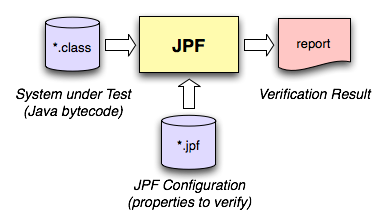
\includegraphics[scale=0.5]{pics/jpf-basic.png} \end{center}
\end{frame}


\begin{frame}[fragile, t]{We are not going to Mars literally, aren`t we?}

Framework from NASA Ames Research Center.

\pause 
\only<2>{
{\small  \url{https://www.nasa.gov/centers/ames/news/releases/2005/05_28AR.html} }
\begin{quote}
JPF was used to detect inconsistencies in the executive software for the K9 Rover at NASA Ames. The K9 rover is a six-wheeled, solar-powered rover developed jointly at NASA Ames and NASA's Jet Propulsion Laboratory
\end{quote}


\begin{center} 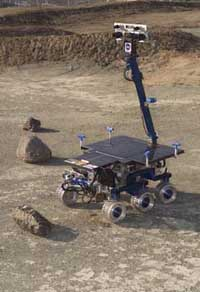
\includegraphics[scale=0.5]{pics/k9-rover.jpg} \end{center}
}

\pause

{\small \url{https://www.nasa.gov/centers/ames/news/releases/2005/05_28AR.html} }
{\small \url{https://en.wikipedia.org/wiki/Earth_Observing-1} }

\begin{quote}
 ... scientists used elements of JPF to develop verification computer code for Livingstone 2 software, a diagnosis system now flying on the EO-1 spacecraft.
\end{quote}

\begin{center} 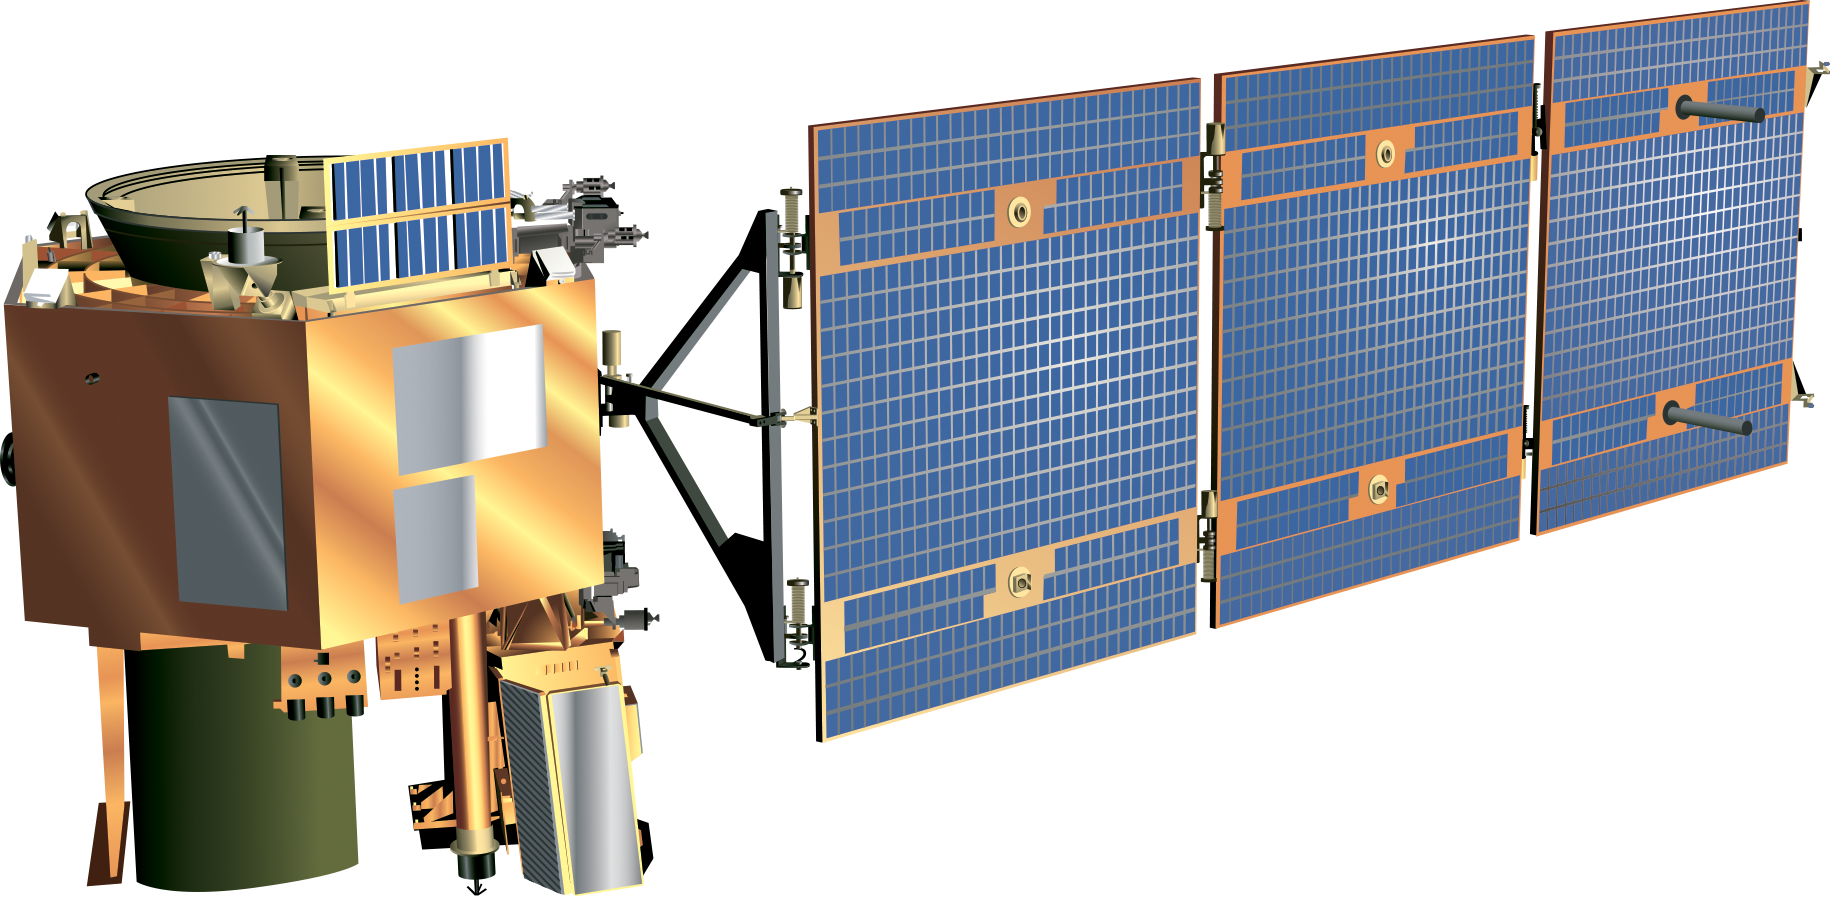
\includegraphics[scale=0.5]{pics/Eo1.png} \end{center}
\end{frame}

\begin{frame}[t,fragile]{Homework: rocket science}

{\small\url{https://github.com/Svazars/parallel-programming/tree/main/hw/block1/6.3}}
\begin{homeworkmail}{Task 6.3}
    \begin{itemize}
        \item Get familiar with JPF, Task 1.2 (almost) solved automatically        
        \item Finish it!
    \end{itemize}
\end{homeworkmail}

{\small\url{https://github.com/Svazars/parallel-programming/tree/main/hw/block1/6.4}}
\begin{homeworkmail}{Task 6.4}
    \begin{itemize}
        \item Solve Task 1.3 using JPF        
    \end{itemize}
\end{homeworkmail}

\end{frame}

\begin{frame}[t,fragile]{Concurrent reliability is hard}
\begin{itemize}
  \item \alarmOne
  \item \alarmTwo
  \item \alarmThree
  \item \alarmFour
  \item \alarmFive
  \item \alarmSix
  \item \alarmSeven
\end{itemize}
\end{frame}

\begin{frame}[t,fragile,noframenumbering]{Concurrent reliability is hard?}
\begin{itemize}
  \item \alarmOne
  \item \alarmThree  
\end{itemize}
\end{frame}

\begin{frame}[t,fragile]{Automation of automation}
\url{https://en.wikipedia.org/wiki/Clarke\%27s_three_laws}
\begin{quote}
  Any sufficiently advanced technology is indistinguishable from magic
\end{quote}

\pause

\begin{itemize}
  \item Tools that automatically generate concurrent tests for my classes?  
\end{itemize}
\end{frame}

\begin{frame}[t,fragile,noframenumbering]{Automation of automation}
\url{https://en.wikipedia.org/wiki/Clarke\%27s_three_laws}
\begin{quote}
  Any sufficiently advanced technology is indistinguishable from magic
\end{quote}

\begin{itemize}
  \item Tools that automatically generate \textbf{reliable} concurrent tests for my classes?
  \pause \item Tools that find visibility bugs without running various software/hardware configurations?
\end{itemize}
\end{frame}

\questiontime{Do you believe in Compute Science magic?}

\begin{frame}{Supernatural tools: lincheck}

{\small\url{https://kotlinlang.org/docs/lincheck-guide.html}}
\begin{itemize}
  \item Creates \textbf{concurrent} tests for your data structure
  \item Runs multithreaded stress-tests
  \item Explores possible interleavings via bounded model checking
\end{itemize}

\pause

\begin{quote}
  Verifies that the results of each invocation satisfy the required correctness property (linearizability is the default one).
\end{quote}

\pause
{\small\url{https://kotlinlang.org/docs/progress-guarantees.html}}
\begin{quote}
  ... wait-freedom ... lock-freedom ... obstruction-freedom
\end{quote}

\pause
{\small\url{https://kotlinlang.org/docs/sequential-specification.html}}
\begin{quote}
  To be sure that the algorithm provides correct sequential behavior, you can define its sequential specification
\end{quote}
\end{frame}

\begin{frame}[t,fragile,noframenumbering]{Concurrent reliability is hard?}
\begin{itemize}
  \item \alarmOne
  \item \alarmThree  
\end{itemize}
\end{frame}

\begin{frame}[t,fragile]{Supernatural tools: herd}

{\small\url{https://diy.inria.fr/www/}}

\begin{minted}{text}
 AArch64 MP
 ---------------------------
 P0          | P1          ;
 MOV W0,#1   | LDR W0,[y]  ;
 STR W0,[x]  | LDR W2,[x]  ;
 MOV W2,#1   |             ;
 STR W2,[y]  |             ;
exists
(P1:W0=1 /\ P1:W2=0)
\end{minted}

\pause
How he knows which loads and stores AArch64 CPU is allowed to reorder?

\pause
Such analysis could be run even in \textit{my browser}?

\end{frame}


\begin{frame}[t,fragile,noframenumbering]{Supernatural tools: herd}

{\small\url{https://github.com/herd/herdtools7}}
\begin{itemize}
 \item generic simulator for weak memory models
 \item produce litmus tests from concise specifications
 \item run litmus tests to test the memory model of the executing machine
\end{itemize}

\pause
{\small\url{https://diy.inria.fr/newdoc/herd.html}}
\begin{quote}
The non-SC behaviour is now accepted, as write-to-read po-pairs do not participate to the acyclicity check any more. In effect, this allows the last execution above, as ghb (i.e. po-tso | com-tso) is acyclic. 
\end{quote}

\begin{center}
 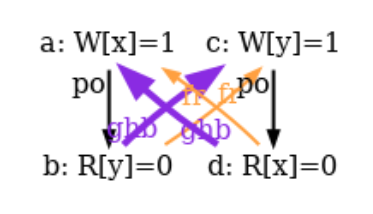
\includegraphics[width=0.3\textwidth]{./pics/herd-sample.png}
\end{center}
 
\end{frame}


\begin{frame}{Supernatural tools: to use or not to use?}

Concurrency-targeted tools could do all the heavy lifting
\begin{itemize}
  \item Create concurrent tests for specified data structure
  \item Enumerate all possible interleavings for particular test 
  \begin{itemize}
      \item show execution trace for any found defect
  \end{itemize}
  \item Reliably detect weak memory model quirks
  \begin{itemize}
      \item no need to buy arm32+aarch64+power CPUs to reproduce
  \end{itemize}
\end{itemize}

\pause
Such tools expect you to have broad context
\begin{itemize}
  \item concurrent consistency, sequential specification, linearizability
  \item read-modify-write, wait-free, lock-free, obstruction-free  
  \item cache coherency, weak memory model, memory barriers, litmus tests
  \item visibility, language memory model
\end{itemize}

\pause
Looks like a plan for second block of this course!
\end{frame}

%\begin{frame}{Chaos mode}
%
%\begin{itemize}
%  \item Multi-threaded program executed by single processor (pre-emptive multitasking)
%  \item Every scheduling decision is
%  \begin{itemize}
%    \item Reproducible 
%    \item Customizable -- pseudo-random with some seed
%  \end{itemize}
%\end{itemize}
%
%\pause
%Advantages:
%\begin{itemize}
%  \item Helps to find/reproduce race conditions, data races, deadlocks
%\end{itemize}
%
%\pause
%Disadvantages:
%\begin{itemize}
%  \item Subtle concurrency problems (word tearing, visibility) are not detected
  %\item Heuristic search of "interesting"\ scheduling decisions\footnote{\tiny{Probabilistic Guarantees of Finding Bugs \ }\tiny\url{https://www.microsoft.com/en-us/research/wp-content/uploads/2016/02/asplos277-pct.pdf}}
%\end{itemize}
%
%\end{frame}


% \section{Failure analysis}
% 
% \begin{frame}{Diagnostics}
% 
% When problem already happened
% - assertions/descriptive exceptions
% - useful logs (always enabled, lightweight?)
% - observability APi (jstack, jmap, access to machine). Netflix experience of brendan gregg
% - TRIVIAL_MODE switch in source code (make your customers a favour) -- tremendously helps to limit debugging scope
% - make your best to create regression scenario in CI/CD
% 
% \end{frame}


\section{Summary}

\begin{frame}{Reliable concurrent software: chasing the horizon}

Any error must manifest itself as soon as possible:
\begin{itemize}
  \item Readable and complete documentation, locking policy, inheritance suggestions
  \item External invariants (exceptions) + internal invariants (assertions)
\end{itemize} 

Use as many validation techniques as you could:
\begin{itemize}
  \item Unit testing
  \item Stress testing
  \item Estimate bug propability and required post-fix testing effort
\end{itemize} 

Master tools:
\begin{itemize}
  \item Test generation
  \item Static checks
  \item Dynamic checks  
  \item Scheduling randomization
  \item Bounded model checking
\end{itemize}
\end{frame}


%\begin{frame}{Algorithm correctness}
%
%Use pen and paper to prove some properties.
%
%\pause
%
%We will discuss required mathematics in Lecture~\foundationsNum \ and Lecture~\foundationsPlusNum.
%
%\end{frame}
%
%
%\begin{frame}{Machine-assisted deductive verification}
%
%Provers and verifiers:
%\begin{itemize}
%  \item Coq \url{https://coq.inria.fr}
%  \item Agda \url{https://wiki.portal.chalmers.se/agda/pmwiki.php}
%  \item PVS \url{https://pvs.csl.sri.com/}
%  \item Z3 \url{https://github.com/Z3Prover/z3}
%\end{itemize}
%
%\pause
%
%There are dedicated courses on formal verification in NSU or Computer Science Center. Which are $N$ times harder than "just programming".
%
%\pause
%
%Software foundations\footnote<3->{\tiny\url{https://softwarefoundations.cis.upenn.edu/}} is $N$ times harder than SICP\footnote<3->{\tiny\url{https://en.wikipedia.org/wiki/Structure_and_Interpretation_of_Computer_Programs}}.
%
%\end{frame}


\begin{frame}{Summary: homework}
    \texttt{Lecture 6, Tasks 6.*:} {\tiny\url{https://github.com/Svazars/parallel-programming/blob/main/hw/block1}}
\end{frame}

\end{document}
